\section{Structure of a RASD document}

The Requirements and Specifications Document (RASD) serves several purposes:
\begin{itemize}
    \item Communication: it conveys an understanding of the requirements, encompassing the application domain and the system under development.
    \item Contractual: it can be legally binding, serving as a formal agreement between stakeholders.
    \item Baseline for project planning and estimation: it provides a foundation for project planning and estimation, covering aspects like size, cost, and schedule.
    \item Baseline for software evaluation: it supports system testing, verification, and validation activities. 
        It contains the information necessary to verify if the delivered system aligns with the requirements.
    \item Baseline for change control: it establishes a foundation for managing changes in requirements as the software evolves.
\end{itemize}
The RASD document is utilized by various stakeholders, including:
\begin{itemize}
    \item Customers and Users: they are interested in a high-level description of system functionalities and requirements.
    \item System analyst and requirement analysts: these individuals use the RASD to specify how the system interacts with other systems.
    \item Developers and programmers: they refer to the RASD for implementation details.
    \item Testers: they use the RASD to check if the system meets its requirements.
    \item Project managers: they rely on the RASD to control the development process.
\end{itemize}
\begin{figure}[H]
    \centering
    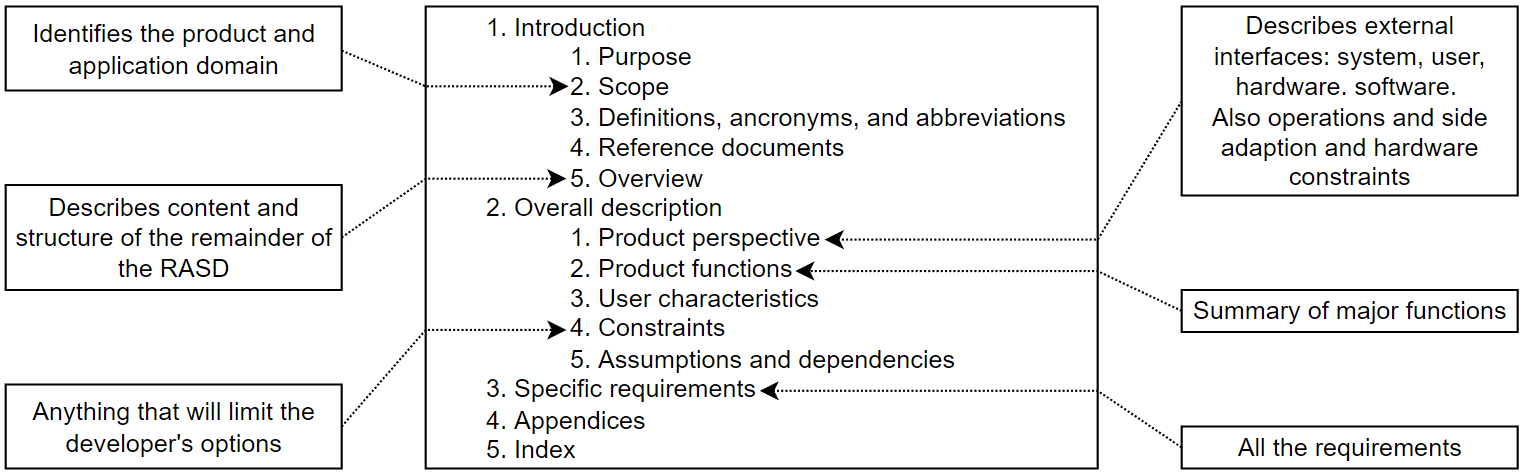
\includegraphics[width=0.75\linewidth]{images/RASD.png}
    \caption{IEEE standard for RASD}
\end{figure}
    
A well-crafted RASD should possess the following qualities:
\begin{itemize}
    \item Completeness:
        \begin{itemize}
            \item Regarding goals: all requirements must satisfy the goals within specified domain assumptions.
            \item Regarding inputs: software behavior should be specified for all possible inputs.
            \item Structural completeness. 
        \end{itemize}
    \item Pertinence: 
        \begin{itemize}
            \item Each requirement or domain assumption should be necessary for achieving a goal.
            \item Each goal should be genuinely needed by the stakeholders.
            \item The RASD should not contain items unrelated to requirement definitions.
        \end{itemize}
    \item Consistency: there should be no contradictions in the formulation of goals, requirements, and assumptions.
    \item Unambiguity: 
        \begin{itemize}
            \item Clear and well-defined vocabulary.
            \item Unambiguous assertions. 
            \item Verifiability of requirements.
            \item Clear delineation of responsibilities between the software and its environment.
        \end{itemize}
    \item Feasibility: the goals and requirements must be achievable within the allocated budget and schedules.
    \item Comprehensibility: the RASD should be easily understandable by the target audience.
    \item Good structuring: every item must be defined before it is used.
    \item Modifiability: the document should be adaptable, and the impact of modifications should be assessable.
    \item Traceability: 
        \begin{itemize}
            \item Indication of the sources of goals, requirements, and assumptions.
            \item Linking requirements and assumptions to underlying goals.
            \item Facilitating referencing of requirements in future documentation.
        \end{itemize}
\end{itemize}   
This structured RASD document ensures effective communication and clarity while serving as a contractual and foundational reference throughout the software development process.
